%! Author = a
%! Date = 12/5/24

\subsection{Metrics comparison}\label{subsec:reward-comparison}
The collider was successfully trained with both negative and rendezvous distance.
Both reward functions performed well in environment with newly pretrained pathfinder.
\begin{figure}[H]
	\centering
	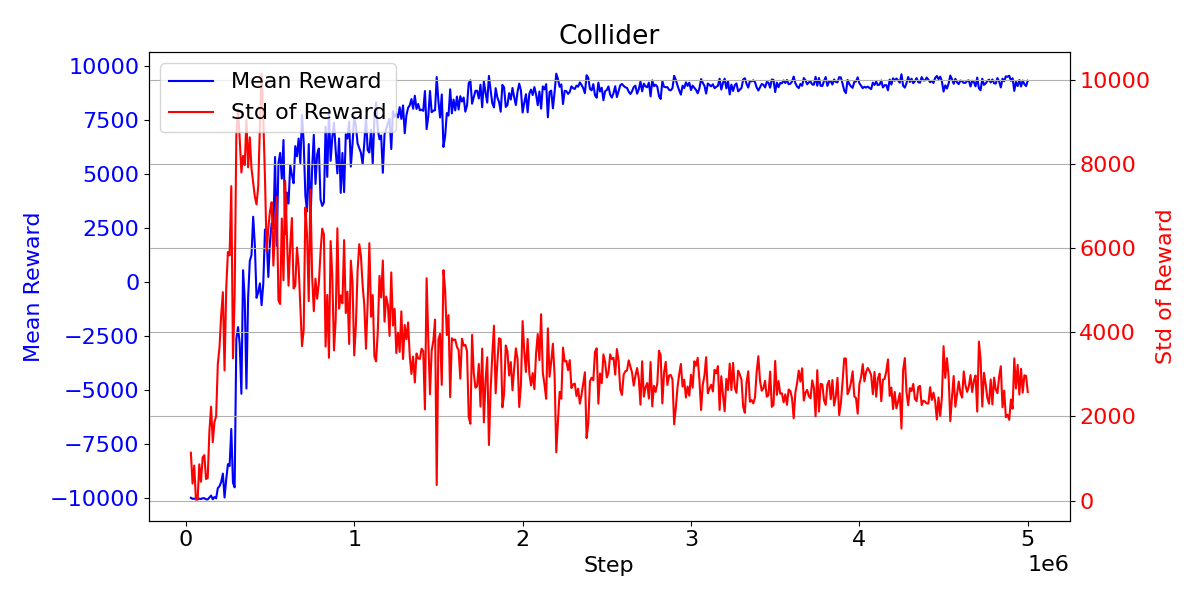
\includegraphics[width=0.5\textwidth]{images/collider_plot.png}
	\caption{Mean and std of the collider reward}
	\label{fig:collider_reward}
\end{figure}
As it can be seen from \ref{fig:collider_reward}, the collider reward mean starts from -10,000 (penalty for leaving the bounding sphere).
As training progresses, the average reward for the collider increases, while that for the pathfinder decreases \ref{fig:pathfinder_reward}, indicating that the collider is successfully intercepting it.
Finally, collider reward reaches +10,000 (reward for intercepting the pathfinder), while pathfinder reward is getting closer to 0.
\begin{figure}[H]
	\centering
	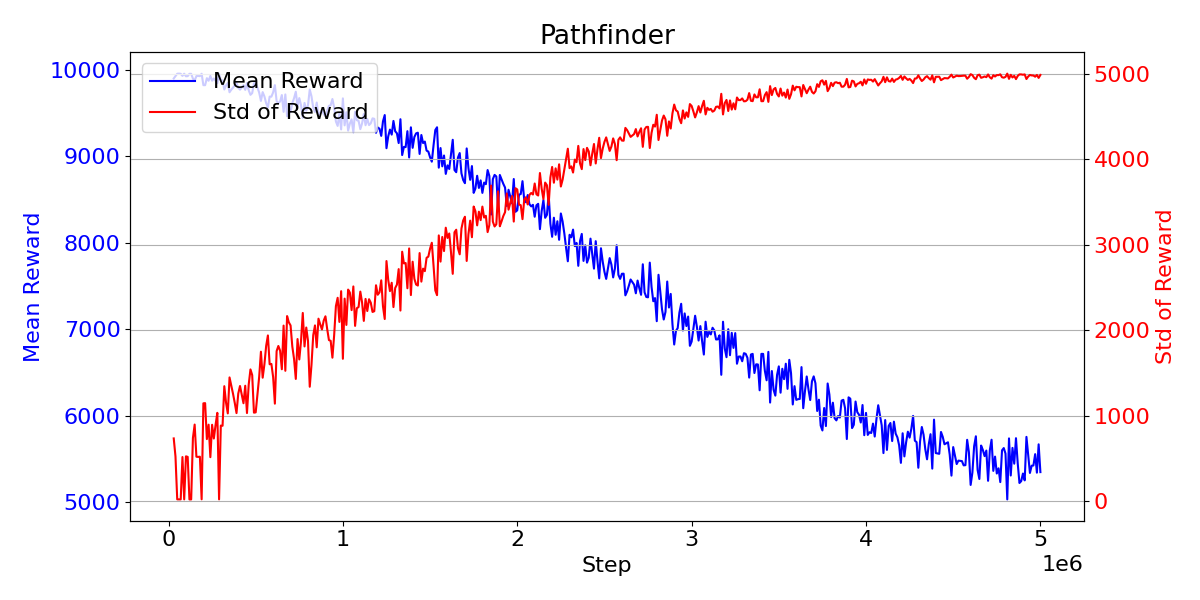
\includegraphics[width=0.5\textwidth]{images/pathfinder_plot.png}
	\caption{Mean and std of the pathfinder reward}
	\label{fig:pathfinder_reward}
\end{figure}

\subsection{Rendezvous vs Negative distance rewards}\label{subsec:rendezvous-vs-negative-distance-rewards}
We were also interested which reward leads to better results: rendezvous or simple negative.
To figure it out, we ran ~5000 simulations with each agent.

Rendezvous distance shows slightly better results.
During the simulations, we saw that agent trained with rendezvous distance reward, easily approaches the pathfinder from different directions, however, bypasses it being extremely close to the target.
The reward function might be improved in the future by introducing separate reward for cases when the collider is close to the target.

\subsection{Screenshots}
Here are some of the screenshots of our simulations.
Blue and red tetrahedrons are collider and pathfinder.
Their predicted trajectories are shown as red and blue lines.
Green spheres represent the predicted points of minimal distance between the agents.

\begin{figure}[H]
	\centering
	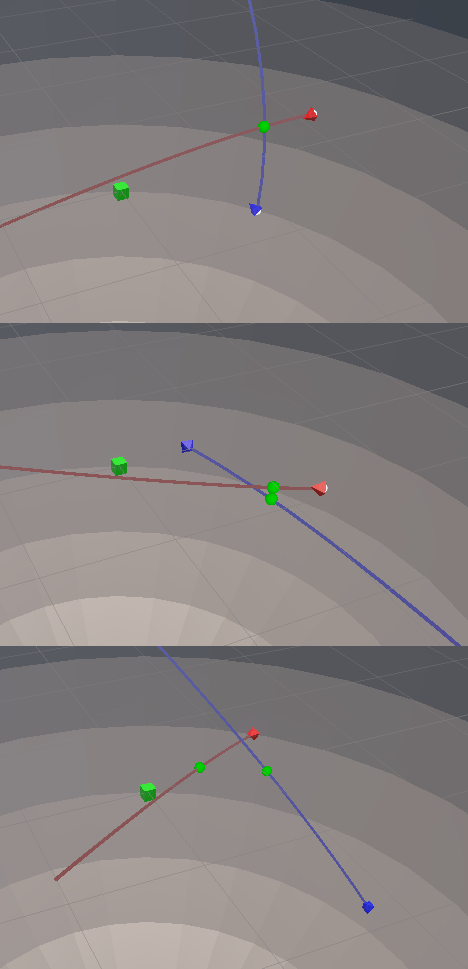
\includegraphics[width=0.3\textwidth]{images/AAA.png}
	\caption{Trajectories and predicted collisions}
	\label{fig:}
\end{figure}